\documentclass[journal]{IEEEtran}

\usepackage{cite}
\usepackage{hyperref}
\usepackage{graphicx}

\usepackage{amsmath}
\interdisplaylinepenalty=2500

\usepackage{listings}
\lstset{basicstyle=\ttfamily\small, breaklines=true}

% correct bad hyphenation here
\hyphenation{op-tical net-works semi-conduc-tor}

\usepackage{xcolor}

\usepackage{listings}
\lstset{escapeinside={<@}{@>}}
\usepackage{color}

\definecolor{dkgreen}{rgb}{0,0.6,0}
\definecolor{gray}{rgb}{0.5,0.5,0.5}
\definecolor{mauve}{rgb}{0.58,0,0.82}

\lstset{frame=tb,
  language=Python,
  aboveskip=3mm,
  belowskip=3mm,
  showstringspaces=false,
  columns=flexible,
  basicstyle={\small\ttfamily},
  numbers=none,
  numberstyle=\tiny\color{gray},
  keywordstyle=\color{blue},
  commentstyle=\color{dkgreen},
  stringstyle=\color{mauve},
  breaklines=true,
  breakatwhitespace=true,
  tabsize=3
}

\begin{document}

\title{Using Fuzzy Logic for extracting department from email content}
\author{Peter Heemskerk, Stefan Schenk, Jim Kamans\\11988797, 11881798, 10302905}

% The paper headers
\markboth{Using Fuzzy Logic for extracting department from email content}{}

\maketitle

\begin{abstract}
Large organizations often struggle to deliver emails or form emails to their corresponding departments if they are not directly addressed to a department or employee. In this project a Fuzzy Logic approach is proposed for automatically determining the correct department. 

A basic version of the approach is implemented with fuzzy logic. The set-up makes it possible to add more flexibility to determine departments not only on content based features but also based on more general features of the email content. 

\end{abstract}

\section{Introduction}
\IEEEPARstart{M}{any} large organizations suffer from their own complexity. If an external party seeks contact with a specific person in an organization, this usually works fine, but if a party seeks contact about a subject (without knowing whom to talk to), it usually takes more time before the party gets a good answer, simply because it is not clear what the right department is which should reply on such a message. At this moment emailing is the main way of communication to businesses, 120 billion emails a year are sent which figure includes a large portion of spam mail \cite{email_statistics}.\\

%\subsection{Problem}

This project aims to solve this issue of low customer service in a complex organization. We present software based on fuzzy logic which aims to bring a message of an external party to the correct internal department purely based on the content of the message.

This project aims to demonstrate that Fuzzy Logic has advantages toward other methods. Firstly, fuzzy logic deals well with incomplete data. Since there is a variety of email messages, short and long, specific and vague, fuzzy logic better deals with these different sources. Secondly, fuzzy logic uses linguistic terms, allowing to include expert knowledge into the system which is relatively easy to interpret.

%\subsection{Objectives}

The goal is determining the correct department from email content. Based on the cleaned word lists a feature vector will be determined for each email. For department determination content specific features are used. These features are used as inputs in the fuzzy logic system to finally determine as output the correct department. Our results will be compared to the given labels of the data-set.\\

\section{Literature reviews}

Fuzzy Logic has been used earlier for email classification. Ferolin \cite{phishing}
has used fuzzy logic to implement a anti-phishing tool using content- and non-content email parameters. A RIPPER Classification Algorithm is used to learn relations of different phishing features, which translate into Fuzzy Logic rules. Santhi et al \cite{spam} determined the degree of dangerousness of spam email with a different method. A Fuzzy Logic system is used to categorize words that are spam in the degree to which these words are considered dangerous. The words are labeled to five linguistic variables which are input for the fuzzy logic algorithm. Ferolin \cite{ranking} introduced a fuzzy logic based ranking function for efficient Information Retrieval. A fuzzy approach was used to rank words based on term-weighting schemes such as term frequency, inverse document frequency and normalization. The term frequency and inverse document frequency and normalization of the query and document are fed to their Fuzzy Logic Controller, whose outputs are fed to the main Fuzzy Logic Controller, which outputs a relevance score. None of these has utilized fuzzy logic for determining departments.

Douglass \cite{ranking} developed an email priority setting learning system for G-mail based on social, content, search label features. These features are use in a statistical model which is parametrized for each user (recipient) separately. This research does not present a solution for situations in larger organizations where there is no information about the individual recipient.

\section{Approach}
For our department determination we follow the procedures proposed by Ferolin for Information Retrieval. The following approach is followed. After data-pre-processing the email words are ranked, resulting in a feature score per email. Words are ranked using a pre-compiled list of words. Then fuzzy logic is applied to classify the email to the correct department.

\subsection{Data}

A private dataset from ``Gemeente Amsterdam'' is used, containing 3371 emails with complaints from citizens.
This dataset is a csv-file where each email has a correct department label, a description of the complaint, a description of contact with an employee and a proposed solution.
An example:
\begin{lstlisting}
Parkeren;Vrijdag voor een ...;Ja, contact
gezocht ...;De 23 euro ...
\end{lstlisting}

\subsection{Feature word-list preparation}

In order to create a feature score for each email (refer to subsection \nameref{subsec:ranking}), feature word-lists are necessary. Other predefined sets of words within the set of relevant words share the same characteristics. For example a set $T \subseteq R$ exists where $T$
is the set of technical words, and $R$ is the set of relevant words from before. Feature list of technical words: $T = [t_1, t_2, \dots, t_n]$.
Other feature lists contain other themed words: $U$, $V$, $W$, \dots .

Feature word-lists are created using the term-frequency / inverse-document-frequency (tf-idf) method. \colorbox{yellow}{ hier nog referentie toevoegen, Jim ?} \colorbox{yellow}{Wil je een algemeen paper over tf-idf hebben of een link naar} \colorbox{yellow}{implementation hoe wij het toepassen?} From the corpus of training emails with the specific department label the following values are calculated for each term. 
\begin{center}
    $tdifd(t) = tf(t) * idf(t)$,
\end{center}
where tf(t) equals the count of terms t, and idf(t) give a ranking of the importance of the word t in the whole corpus: 
\begin{center}
    $idf(t, D) = log\dfrac{N(D)}{n_t(D)}$, 
\end{center}
where $N(D)$ is the total number of documents and $n_t(D)$ equals the number of documents containing the specific term. 
Selecting those terms with a $tdifd > treshold$, the feature-word lists are created, with signal words for the specific department.

\subsection{Data preprocessing}
The data needs to be cleaned and filtered.

\begin{enumerate}
    \item Cleaning

    As an email body is read from the file system as plain text, individual terms are stored as individual values (``tokenized''). After that, capital characters are converted to lower case, punctuation and special characters are removed, stop-words are removed and the words are reduced to their base root form (``stemmed'').

    \item Filtering

    The next operation will perform an intersection between the words and a list of predefined relevant words. Words that are not contained in the word list are removed. As the last filtering step, the words are counted, and a corpus is created.

\end{enumerate}

\subsection{Ranking}
\label{subsec:ranking}
For this experiment the content type of feature determines the subject of the email.

For every word in the email that is present in $T$, a score is calculated that takes the count of that word into account in relation to the total number of relevant words in the email. This calculation is made for all feature lists ($T$, $U$, $V$, $W$), for every word in the email. 

So for each email a feature vector is determined, containing the score between 0 and 1 against the features, as defined by the feature word-lists. 

\subsection{Classification with Fuzzy Logic}

For determining the output variable department four content input variables are defined, corresponding with the content features. Refer to \autoref{table:1}. Since these are mostly chosen as a default, also now for each of the input variables 3 triangular membership functions (ms) are chosen to represent a low, medium or high value. For the output, a variable is created for each of the four departments, each variable containing 3 triangular membership functions low, medium, high.

We have set a rule base for determining departments based on the content input variables. An overview of Rules you can find in \nameref{sec:rules}

\begin{figure}
	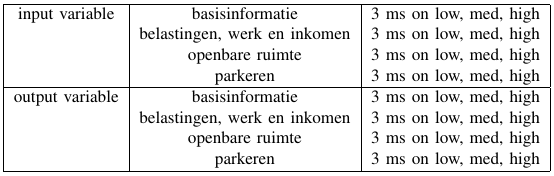
\includegraphics[scale=0.6]{res/inputs_outputs_FLS.png}
	\caption{Input and Output variables in Fuzzy Logic System}
	\label{table:1}
\end{figure}

%\begin{center}
%\begin{tabular}{ |c|c|c| }
% \hline
% input variable & basisinformatie   & 3 ms on low, med, high    \\
%                & belastingen, werk en inkomen & 3 ms on low, med, high \\
%                & openbare ruimte   & 3 ms on low, med, high    \\
%                & parkeren          & 3 ms on low, med, high    \\
% \hline
% output variable& basisinformatie   & 3 ms on low, med, high    \\
%                & belastingen, werk en inkomen & 3 ms on low, med, high \\
%                & openbare ruimte   & 3 ms on low, med, high    \\
%                & parkeren          & 3 ms on low, med, high    \\
%\hline
%\end{tabular}
%\label{table:1}
%Input and Output variables in Fuzzy Logic System
%\end{center}


\subsection{Training and validation}

For training and validation the data set is divided in a training set and validation set with a factor 0.7.

The training set of emails is used for the creation of the feature word-lists using tf/idf. The setting of the Fuzzy Logic rule base is done based on the expert vision of one of the team-members. 

The validation set including the department label is used for validation. 

\subsection{Implementation}

For cooperation purposes we used Github \footnote{\url{https://github.com/Menziess/Fuzzy-Logic-Email-Classification}} (for source control) and Trello \footnote{\url{https://trello.com/fuzzylogicemailclassification}} (as scrum projectmanagement tool)

We used Python3 as programming language and Jupyter Notebook as development
environment. The code is enlisted in \nameref{sec:python}. For data-preprocessing Pythons NLTK module \footnote{\url{http://www.nltk.org/}} is used. For classification a new algorithm has been developed. The fuzzy logic system itself is based on the Fuzzy Logic LAB \footnote{\url{https://blackboard.uva.nl/webapps/blackboard/execute/content/file?cmd=view&content_id=_6947429_1&course_id=_212301_1&framesetWrapped=true}}, amended for using more than one output, a centroid defuzzifier and some more flexibility and error handling in management of fuzzy logic rules.

\section{Experiment}

\subsection{Results}

The automatic process of feature word-list creation, data-preprocessing, ranking and classification with fuzzy logic has been implemented. The process is tested and works.

Validating the calculated departments with known labels has resulted in a 46.2 percent correctness.

\subsection{Discussion}

The project resulted in a baseline for the proposed approach. A feature vector is used which corresponds to the departments already, and we included a basic fuzzy logic implementation. Inclusion of a feature vector has an important advantage that also non-content features (like: ``press sensitive'') can be extracted which may result in determining a different department. The creation of a relevant feature vector based on a large email training set is work to do. 

The fuzzy logic implementation has been basic. We included the feature scores of an e-mail as input, with basic triangular membership functions for low, medium and high. A basic rule set is included, with rules like IF input feature ``parkeren'' is high THEN output department ``parkeren'' is high. Work to do is to learn rules from a training data-set. For this the RIPPER algorithm, or others like Decision Tree or Neural Network may be considered. \cite{rulelearning}\cite{ripper}\\
 
The low classification success percentage is due to the used features and the rules. When looking at the ranking of the training set, no clear rules were found. Each feature has a high score for ``openbare ruimte'', so when ``openbare ruimte'' is high, it can still be any department. It would be better to find features where a high score for that feature would result in only one or two departments. 

\section{Acknowledgment}

This work is done as part of the autumn 2017 bachelor course Fundamentals of Fuzzy Logic by A. Bilgin (and  M. Hol and V. Dankers) within the study Artificial Intelligence at University of Amsterdam.

\begin{thebibliography}{9}
\bibitem{email_statistics}
    The Radicati Group, inc.(2015),
    \textit{
        \href{https://github.com/Menziess/Fuzzy-Logic-Email-Classification/raw/master/report/res/a_new_fuzzy_logic_based_ranking_function_for_efficient_information_retrieval_system.pdf}{Email Statistics Report, 2015-2019},
    }.

\bibitem{spam}
    G.Santhi, S. Maria Wenish, Dr. P. Sengutuvan (2013),
    \textit{
        \href{https://github.com/Menziess/Fuzzy-Logic-Email-Classification/raw/master/report/res/a_content_based_classification_of_spam_mails_with_fuzzy_word_ranking.pdf}{A Content Based Classification of Spam Mails with Fuzzy Word Ranking},
    }
    Department of Information Science and Technology,
    Issue 3.

\bibitem{phishing}
    Rosana J. Ferolin, (2010 - approx.)
    \textit{
        \href{https://github.com/Menziess/Fuzzy-Logic-Email-Classification/raw/master/report/res/a_proactive_anti-phishing_tool_using_fuzzy_logic_and_ripper_data_mining_classification_algorithm.pdf}{A Proactive Anti-Phishing Tool Using Fuzzy Logic and RIPPER Data Mining Classification Algorithm},
    }
    Department of Computer Engineering University of San Carlos.

\bibitem{ranking}
    Rosana J. Ferolin, (2014)
    \textit{
        \href{https://github.com/Menziess/Fuzzy-Logic-Email-Classification/raw/master/report/res/a_new_fuzzy_logic_based_ranking_function_for_efficient_information_retrieval_system.pdf}{A new fuzzy logic based ranking function for efficient Information Retrieval system},
    }
    Department of Electrical Engineering Dayalbagh Educational Institute.

\bibitem{priority}
    Douglas Aberdeen, (2010 approx.)
    \textit{
        \href{[nog toevoegen}{The Learning behind Gmail Priority Inbox}
    }

\bibitem{rulelearning}
    J. Foernkranz, D. Gamberger, N. Lavrac (2012)
    \textit{
        \href{[nog toevoegen}{Foundations of Rule Learning, chapter 2, Rule Learning in a nutshell.}
    }

\bibitem{ripper}
    M. Britsch, N. Gagunashvili, M. Schmelling (2008)
    \textit{
        \href{[nog toevoegen}{Application of the rule-growing algorithm RIPPER to particle physics analysis}
    }

\end{thebibliography}

\newpage

\section*{Attachment A: Rules}
\label{sec:rules}
\noindent
f1, d1 = Basisinformatie\\
f2, d2 = Belasting, Werk en Inkomen\\
f3, d3 = Openbare Ruimte\\
f4, d4 = Parkeren\\

\noindent
IF f1 = low THEN d1 = low\\
IF f1 = med THEN d1 = med\\
IF f1 = high THEN d1 = high\\
IF f2 = low THEN d2 = low\\
IF f2 = med THEN d2 = med\\
IF f2 = high THEN d2 = high\\
IF f3 = low THEN d3 = low\\
IF f3 = med THEN d3 = med\\
IF f3 = high THEN d3 = high\\
IF f4 = low THEN d4 = low\\
IF f4 = med THEN d4 = med\\
IF f4 = high THEN d4 = high\\
IF f1 = low and f2 = low and f3 = low and f4 = low THEN d1 = high

\newpage

\section*{Attachment B: Python code}
\label{sec:python}

\subsection*{main.py}
\begin{lstlisting}
def main():

	# Parameters to easily tune stuff
	params = {

		'limit'		: None, 		# None / 1231
		'verbose'	: True, 		# True / False
		'defuz' 	: "centroid",	# "centroid", "lom", "som"
		'trial'		: "max",		# "max", "rel", "high"

		'delimiter' : ';',

		'print_results': False,
		'results_path': "res/results.txt",

		'datadump' 	: "res/klachtendumpgemeente.csv",
		'validdump' : "res/validationdump.csv",
		'traindump' : "res/traindump.csv",
		'features' 	: "res/categories/*.csv",
		'word_list' : "res/categories/word_list/word_list.csv",

	}

	# Read validation data
	dump = read_csv(params['validdump'],
					params['delimiter'])

	# Create rate object that creates
	# feature vectors for all emails
	rater =   Rater(params['features'],
					params['word_list'])

	# Lists with features used by the
	# rater object to rate the emails
	feature_lists = rater.feature_lists

	# Rows and rated generators to iterate
	# through rated and non-rated emails
	rows = ((row[0], tokenize(row[1])) for row in dump[1:])
	rated = ((row[0], row[1], rater.rate_email(row[1])) for row in rows)

	# Inputs for the Fuzzy Logic System
	inputs = [

		Input(feature[0], (0, 1), [
			TrapezoidalMF("low", -.2, -.1, 0, 0.5),
			TriangularMF("med", 0, 0.5, 1),
			TrapezoidalMF("high", 0.5, 1, 1.1, 1.2)
		]) for feature in feature_lists

	]

	# Outputs for the Fuzzy Logic System
	outputs = [

		Output(feature[0], (0, 1), [
			TrapezoidalMF("low", -.2, -.1, 0, 0.5),
			TriangularMF("med", 0, 0.5, 1),
			TrapezoidalMF("high", 0.5, 1, 1.1, 1.2)
		]) for feature in feature_lists

	]

	# Rules for the Fuzzy Logic System
	rules = [

		Rule(1, ["high", "", "", ""],
			"and", ["high", "", "", ""]),
		Rule(2, ["med", "", "", ""],
			"and", ["med", "", "", ""]),
		Rule(3, ["low", "", "", ""],
			"and", ["low", "", "", ""]),
		Rule(4, ["", "", "high", ""],
			"and", ["", "", "high", ""]),
		Rule(5, ["", "", "med", ""],
			"and", ["", "", "med", ""]),
		Rule(6, ["", "", "low", ""],
			"and", ["", "", "low", ""]),
		Rule(7, ["", "", "", "high"],
			"and", ["", "", "", "high"]),
		Rule(8, ["", "", "", "med"],
			"and", ["", "", "", "med"]),
		Rule(9, ["", "", "", "low"],
			"and", ["", "", "", "low"]),
		Rule(10, ["", "high", "", ""],
			"and", ["", "high", "", ""]),
		Rule(11, ["", "med", "", ""],
			"and", ["", "med", "", ""]),
		Rule(12, ["", "low", "", ""],
			"and", ["", "low", "", ""]),

		# Catches empties
		Rule(13, ["low", "low", "low", "low"],
			"and", ["high", "", "", ""]),

	]

	# Fuzzy Logic Classifier
	classifier = Classifier(
		inputs, outputs,
		rules, params
	)

	# Analyzes entire or parts of a classification
	# of the validation dataset
	statistics = Statistics(params)
	statistics.start(rated, classifier)

# Cleans plain text into arrays of words
def tokenize(body):
	tokens = word_tokenize(body)
	tokens = [w.lower() for w in tokens]
	tokens = [w for w in tokens if len(w) > 2]
	table = str.maketrans('', '', string.punctuation)
	stripped = [w.translate(table) for w in tokens]
	words = [word for word in stripped if word.isalpha()]
	stop_words = list(get_stop_words('nl'))
	nltk_words = list(stopwords.words('dutch'))
	stop_words.extend(nltk_words)
	words = [w for w in words if not w in stop_words]
	stemmer = SnowballStemmer("dutch")
	words = [stemmer.stem(word) for word in words]
	return words

# Reads comma separated file
def read_csv(filepath, delimiter=','):
	with open(filepath, 'r') as c:
		return [row for row in csv.reader(c, delimiter=delimiter,
			skipinitialspace=True)]

# Compares arrays of words and calculates a score
class Rater:
	def __init__(self, features, word_list):
		self.path = features
		self.word_list = read_csv(word_list)[0]
		self.feature_lists = [
			(os.path.basename(fname).split('.')[0],
			read_csv(fname)[0])
			for fname in glob.glob(self.path)]
		self.feature_lists.sort(key=lambda tup: tup[0])
	def corpus(self, email):
		words = [w for w in email if w in self.word_list]
		return np.c_[np.unique(words, return_counts=True)]
	def rate_words(self, email):
		c = self.corpus(email)
		c_len = len(c)
		for n, f in self.feature_lists:
			c = np.c_[c, np.zeros(c_len)]
			for row in c:
				if (row[0] in f):
					row[-1:] = int(row[1]) / c_len
		return c
	def rate_email(self, email):
		c = self.rate_words(email)
		ratings = dict()
		for i, feature in enumerate(self.feature_lists):
			agg = min(c[:,i + 2].astype(np.float).sum(), 1.0)
			ratings[feature[0]] = float(format(agg, '.2f'))
		return ratings

# Classifies one or bulks of emails
class Statistics:
	def __init__(self, params):
		self.params = params
		self.iterations = 0
		self.success = 0
		self.template = "{label:19.19} | {c:19.19} | {success:7} | {r_list}"
		self.verbose = "score: {guess_score}, opposite: {opposite_score}, relative: {relative_score}"
	def print(self, classification, file):
		if self.params['verbose']:
			print(self.template.format(**classification), file=file)
			print(self.verbose.format(**classification), file=file)
			print(classification['r'], '\n')
		else:
			print(self.template.format(**classification), file=file)
	def push(self, c):
		self.iterations += 1
		if c['correct_guess']:
			self.success += 1
	def start(self, rated, classifier):
		with open(self.params['results_path'], 'w', newline='') as f:
			if not self.params['print_results']:
				f = None
			print("%19s | %19s | %7s | %1s"
				% ("LABEL", "CLASS", "SUCCESS", "RATING"), file=f)
			for i, email in enumerate(rated):
				c = classifier.classify(email)
				self.push(c)
				self.print(c, file=f)
				if self.params['limit'] and i + 1 >= self.params['limit']:
					break
			print("\nTotal Success:", self.success, "/",
				self.iterations,
				"(" + str(round(self.success / self.iterations * 100, 1))
				+ "%)\n", file=f)

			if self.params['trial'] == "max":
				print("Trial 'max': (correctly guessed if class equals label)",
					file=f)
			elif self.params['trial'] == "rel":
				print("Trial 'rel': (correctly guessed if relative > 0.33, "
					+ "enable verbose for more output information)",
					file=f)
			elif self.params['trial'] == "high":
				print("Trial 'high': (correctly guessed if score > 0.75, "
					+ "enable verbose for more output information)",
					file=f)
		if self.params['print_results']:
			print("\nResults printed in file:", self.params['results_path'])

# Imports hidden at the bottom
import os
import csv
import glob
import nltk
import string

nltk.download('punkt')
nltk.download('stopwords')

from many_stop_words import get_stop_words
from nltk.tokenize import word_tokenize
from nltk.corpus import stopwords
from nltk.stem.snowball import SnowballStemmer
from __fuzzy_logic.classifier import *

# Calls main method
if __name__ =='__main__':
	main()
\end{lstlisting}

\subsection*{classifier.py}
\begin{lstlisting}
# Contains Fuzzy Logic System Classes

import math
import numpy as np
from collections import defaultdict, Counter

class Classifier:
	"""Classifier that takes a feature vector as input, produces scalars as output."""
	def __init__(self, inputs, outputs, rules, params):
		self.inputs = inputs
		self.outputs = outputs
		self.rulebase = Rulebase(rules)
		self.params = params
		self.reasoners = dict()
		self.reason()
	def reason(self):
		if (len(self.reasoners) > 0):
			return print("Already reasoned")
		for i, output in enumerate(self.outputs):
			self.reasoners[output.name] = Reasoner(
				self.rulebase,
				self.inputs,
				self.outputs,
				i, 201, self.params['defuz'])
	def classify(self, email):
		# Get email information
		# department, body and ratings
		dept, body, r = email
		# Unpack rating
		r_list = list(r.values())
		# Classify email
		c_list = {
			name : round(reasoner.inference(r_list), 3)
			for name, reasoner in self.reasoners.items()
		}
		# Pick best
		c = max(c_list, key=lambda k: c_list[k])
		guess_score = c_list[dept.lower()]
		opposite_score = round(sum(c_list.values()) - guess_score, 3)
		relative_score = round(guess_score / (opposite_score + 2e-26), 3)

		success = dept.lower() == c.lower()
		if self.params['trial'] == "relative":
			success = relative_score >= 0.33
		elif self.params['trial'] == "high":
		 	success = guess_score >= 0.75

		# Return results where T is succesfullness of classification
		return {
			"success" : str(success),
			"correct_guess" : success,
			"guess_score" : guess_score,
			"opposite_score": opposite_score,
			"relative_score": relative_score,
			"label" : dept,
			"words" : body,
			"r" : r,
			"r_list" : r_list,
			"c" : c,
			"c_list" : c_list,
		}

class TriangularMF:
	"""Triangular fuzzy logic membership function class."""
	def __init__(self, name, start, top, end):
		self.name = name
		self.start = start
		self.top = top
		self.end = end
	def calculate_membership(self, x):
		if x <= self.start:
			y = 0
		if x > self.start and x <= self.top:
			y = (x-self.start)/(self.top-self.start)
		if x > self.top and x <= self.end:
			y = (self.end - x)/(self.end - self.top)
		if x > self.end:
			y = 0
		return y

class TrapezoidalMF:
	"""Trapezoidal fuzzy logic membership function class."""
	def __init__(self, name, start, left_top, right_top, end):
		self.name = name
		self.start = start
		self.left_top = left_top
		self.right_top = right_top
		self.end = end
	def calculate_membership(self, x):
		if x <= self.start:
			y = 0
		if x > self.start and x <= self.left_top:
			y = (x - self.start)/(self.left_top - self.start)
		if x > self.left_top and x <= self.right_top:
			y = 1
		if x > self.right_top and x <= self.end:
			y = (self.end - x)/(self.end - self.right_top)
		if x > self.end:
			y = 0
		return y

class Variable:
	"""General class for variables in an FLS."""
	def __init__(self, name, range, mfs):
		self.name = name
		self.range = range
		self.mfs = mfs
	def calculate_memberships(self, x):
		return {
			mf.name : mf.calculate_membership(x)
			for mf in self.mfs
		}
	def get_mf_by_name(self, name):
		for mf in self.mfs:
			if mf.name == name:
				return mf

class Input(Variable):
	"""Class for input variables, inherits
	variables and functions from superclass Variable."""
	def __init__(self, name, range, mfs):
		super().__init__(name, range, mfs)
		self.type = "input"

class Output(Variable):
	"""Class for output variables, inherits
	variables and functions from superclass Variable."""
	def __init__(self, name, range, mfs):
		super().__init__(name, range, mfs)
		self.type = "output"

class Rule:
	"""Fuzzy rule class, initialized with an antecedent (list of strings),
	operator (string) and consequent (string)."""
	def __init__(self, n, antecedent, operator, consequent):
		self.number = n
		self.antecedent = antecedent
		self.operator = operator
		self.consequent = consequent
		self.firing_strength = 0
	def calculate_firing_strength(self, datapoint, inputs):
		memberships = []

		for a, x, i in zip(self.antecedent, datapoint, inputs):
			if (a == ''):
				memberships.append(0)
				continue

			m = i.get_mf_by_name(a).calculate_membership(x)
			memberships.append(m)

		# Filtering out zero values
		memberships = [x for x in memberships if x]

		if not memberships:
			self.firing_strength = 0

		elif self.operator == "and":
			self.firing_strength = min(memberships)

		elif self.operator == "or":
			self.firing_strength = max(memberships)

		return self.firing_strength

class Rulebase:
	"""The fuzzy rulebase collects all rules for the FLS, can
	calculate the firing strengths of its rules."""
	def __init__(self, rules):
		self.rules = rules
	def calculate_firing_strengths(self, datapoint, inputs, outputindex):
		result = Counter()
		for i, rule in enumerate(self.rules):
			consequent = rule.consequent[outputindex]
			if consequent != "":
				fs = rule.calculate_firing_strength(datapoint, inputs)
				if fs > result[consequent]:
					result[consequent] = fs
			# print(datapoint, rule.antecedent, result[consequent])
		return result

class Reasoner:
	def __init__(self, rulebase, inputs, output, outputindex, n_points, defuzzification):
		self.rulebase = rulebase
		self.inputs = inputs
		self.output = output
		self.outputindex = outputindex
		self.discretize = n_points
		self.defuzzification = defuzzification
	def inference(self, datapoint):
		firing_strengths = self.rulebase.calculate_firing_strengths(
			datapoint, self.inputs, self.outputindex)
		self.check_consequents(firing_strengths)
		input_value_pairs = self.aggregate(firing_strengths)
		crisp_output = self.defuzzify(input_value_pairs)
		return crisp_output
	def aggregate(self, firing_strengths):
		agg_start = self.output[self.outputindex].range[0]
		agg_end = self.output[self.outputindex].range[1]
		aantal = self.discretize
		breedte = (agg_end - agg_start)/(aantal-1)
		input_value_pairs = []
		for n in range(aantal):
			x = agg_start + n * breedte
			mslijst = self.output[self.outputindex].calculate_memberships(x)
			value = 0
			for ms in mslijst:
				ms_min = min(mslijst[ms], firing_strengths[ms])
				value = max(ms_min, value)
			input_value_pairs.append((x, value))
		return input_value_pairs
	def defuzzify(self, input_value_pairs):
		maxms = 0
		crisp_value = -1
		if self.defuzzification =="som":
			for value_pair in input_value_pairs:
				if value_pair[1]>maxms:
					maxms = value_pair[1]
					crisp_value = value_pair[0]
		elif self.defuzzification == "lom":
			for value_pair in input_value_pairs:
				if value_pair[1]>=maxms:
					maxms = value_pair[1]
					crisp_value = value_pair[0]
		elif self.defuzzification == 'centroid':
			teller = 0
			noemer = 0
			for value_pair in input_value_pairs:
				teller += value_pair[0] * value_pair[1]
				noemer += value_pair[1]
			if noemer == 0:
				crisp_value = 0
			else:
				crisp_value = teller / noemer
		return crisp_value
	def check_consequents(self, firing_strengths):
		agg_start = self.output[self.outputindex].range[0]
		mslijst = self.output[self.outputindex].calculate_memberships(agg_start)
		for ms in firing_strengths:
			if ms not in mslijst:
				print('WARNING - consequent:', ms,
					'does not match outputdefinition')
		return
\end{lstlisting}

\subsection*{data\_preparation.py}
\begin{lstlisting}
from __data_preparation.train_validation_splitter import *
from __data_preparation.categories_maker import *

# Dump requires three values: input dump path, validation dump path
# and train dump paths, in that particular order
# The 'threshold' determines wihch minimal tf/idf score is required
# for words to end up in the category lists
params = {
	'threshold' : 0.2,
	'verbose'	: True,
	'delimiter' : ';',
	'train_data_split_factor' : .70,

	'datadump' 	: "res/klachtendumpgemeente.csv",
	'validdump' : "res/validationdump.csv",
	'traindump' : "res/traindump.csv",

	# Currently creating union word_list in categories folder
	# instead of features folder
	'word_list_path' : "res/categories/word_list/",
	'categories_path' : "res/categories/",
	'features_path' : "res/features/",
}

# Splitting datadump into two lists to prevent overfitting
Splitter(params)

# Create lists of cleaned and filtered words for each category
# and a combined list for all distinct words of all categories
# Prompting user to prevent unwanted overwriting of categories
while True:
	print("You're about to write/overwrite category list csv's in \""
		+ params['categories_path']
		+ "\".\nEnter a threshold above 0, if that's what you'd like to do: ")
	try:
		t = float(input("> "))
		params['threshold'] = t
		break
	except ValueError:
		print("Man, learn to type a number.")

Corpus(params)
\end{lstlisting}

\subsection*{categories\_maker.py}
\begin{lstlisting}
import os
import csv
import math
from collections import Counter
from __data_preparation.utils import *

class Tfidf:
	def __init__(self):
		self.n_containing_dict = dict()
	def tf(self, word, row):
		return row.count(word) / len(row)
	def n_containing(self, word, rows):
		if (word in self.n_containing_dict):
			return self.n_containing_dict[word]
		n = sum(1 for row in rows if word in row)
		self.n_containing_dict[word] = n
		return n
	def idf(self, word, rows):
		return math.log(len(rows) / (1 + self.n_containing(word, rows)))
	def tfidf(self, word, row, rows):
		return self.tf(word, row) * self.idf(word, rows)

class Corpus:
	"""Designed to filter meaningfull words from a datadump and store
	the words in a csv file having a corresponding label"""
	def __init__(self, params):
		self.rows = None
		self.categories = None
		self.process(params)

	# Starts steps of creating category lists
	def process(self, params):
		self.read_dump(params)
		self.count_distinct_categories()
		self.tokenize()
		self.filter_categories(params)

	# Reads the train datadump
	def read_dump(self, params):
		with open(params['traindump'], 'r') as c:
			reader = csv.reader(c,
				delimiter=params['delimiter'],
				skipinitialspace=True)
			self.rows = [row for row in reader][1:]

	# Counts distinct categories
	def count_distinct_categories(self):
		self.categories = list(set([row[0] for row in self.rows]))

	# Tokenizes and cleans email bodies
	def tokenize(self):
		for row in self.rows:
			row[1] = tokenize(row[1])

	# Creates lists of words, per category, with tf/idf score above threshold
	def filter_categories(self, params):
		if not os.path.exists(params['categories_path']):
			os.makedirs(params['categories_path'])
		if not os.path.exists(params['word_list_path']):
			os.makedirs(params['word_list_path'])
		word_list = []
		common_word_list = []

		# After folders are created, start tf/idf
		print("Starting tf/idf process, this may take a while...")
		tfidf = Tfidf()
		for category in self.categories:
			print("Category:", category, "- threshold:", params['threshold'])
			rows = [row for row in self.rows if category == row[0]]
			favorite_words = set(self.tfidf(rows, tfidf, params))
			print(category + ":", len(favorite_words))
			word_list += favorite_words
			common_word_list = intersection(common_word_list, favorite_words)
			generate_csv_from_array(params['categories_path'] + category.lower() + ".csv", favorite_words)

		# Creates final word_list, a union set of all category lists
		generate_csv_from_array(
			params['word_list_path'] + "word_list.csv",
			set([x for x in word_list if x not in common_word_list]))

	# Extracts words with tf/idf score above threshold
	def tfidf(self, rows, tfidf, params):
		favorite_words = []
		for i, row in enumerate(rows):
			scores = {word: tfidf.tfidf(word, row[1], [r[1] for r in self.rows]) for word in row[1]}
			best_words = sorted(scores.items(), key=lambda x: x[1],
				reverse=True)
			for word, score in best_words:
				if (score >= params['threshold']):
					if (params['verbose']):
						print("\tWord: {}, TF-IDF: {}".format(word, round(score, 5)))
					favorite_words.append(word)
		return favorite_words
\end{lstlisting}

\subsection*{train\_validation\_splitter.py}
\begin{lstlisting}
import random
from __data_preparation.utils import *

class Splitter:
	"""Splits given dataset into train and validation sets."""
	def __init__(self, params):
		self.split(params)
	def split(self, params):
		data = read_csv(params['datadump'], params['delimiter'])
		t = csv.writer(open(params['traindump'], 'w', newline=''),
			delimiter=params['delimiter'])
		v = csv.writer(open(params['validdump'], 'w', newline=''),
			delimiter=params['delimiter'])

		# Write header
		v.writerow(data[0])
		t.writerow(data[0])

		# Shuffle rest
		data = data[1:]
		random.shuffle(data)

		# Split data based on factor
		f = params['train_data_split_factor']
		train_data = data[:int((len(data)+1) * f)]
		valid_data = data[int(len(data)* f + 1):]

		# Write data to csv files
		[t.writerow(row) for row in train_data]
		[v.writerow(row) for row in valid_data]

		print("Original dump length:", len(data))
		print("Written", len(train_data), "rows to \"" + params['traindump']
			+ "\" and", len(valid_data), "rows to \"" + params['validdump']
			+ "\" used a factor of:", f)
\end{lstlisting}

\subsection*{utils.py}
\begin{lstlisting}
import os
import sys
import csv
import glob
import nltk
import string
import pandas as pd
import numpy as np

nltk.download('punkt')
nltk.download('stopwords')

from many_stop_words import get_stop_words
from nltk.tokenize import word_tokenize
from nltk.corpus import stopwords
from nltk.stem.snowball import SnowballStemmer
from collections import Counter

def tokenize(body):
    """
    Tokenizer.

    Converts plain text to array of tokens.

    Parameters
    ----------
    body : str
        Plain text that is to be cleaned and tokenized.

    Returns
    -------
    List
        A cleaned list of words.

    """
    tokens = word_tokenize(body)
    tokens = [w.lower() for w in tokens]
    tokens = [w for w in tokens if len(w) > 2]
    table = str.maketrans('', '', string.punctuation)
    stripped = [w.translate(table) for w in tokens]
    words = [word for word in stripped if word.isalpha()]
    stop_words = list(get_stop_words('nl'))
    nltk_words = list(stopwords.words('dutch'))
    stop_words.extend(nltk_words)
    words = [w for w in words if not w in stop_words]
    stemmer = SnowballStemmer("dutch")
    words = [stemmer.stem(word) for word in words]
    return words

def read_txt(filepath):
    """
    Plain text reader.

    Reads and cleans a text file located at filepath.

    Parameters
    ----------
    filepath : string
        Location of the file.

    Returns
    -------
    List
        A cleaned list of words.

    """
    with open(filepath, 'r') as file:
        body = file.read()
    return tokenize(body)

def read_csv(filepath, delimiter=','):
    """
    Csv reader.

    Reads csv file.

    Parameters
    ----------
    filepath : str
        Location of the file.
    delimiter : str
        Delimiter character, separating values.

    Returns
    -------
    List
        Containing a list of words for each row.

    """
    with open(filepath, 'r') as c:
        return [row for row in csv.reader(c, delimiter=delimiter,
            skipinitialspace=True)]

def generate_csv_from_array(filename, array):
    """
    Csv from array.

    Writes array to csv file.

    Parameters
    ----------
    filename : str
        Location to write file to.
    array : List
        Array that needs to be written.

    """
    with open(filename, 'w', newline='') as c:
        writer = csv.writer(c, delimiter=',')
        writer.writerow(array)

def intersection(array1, array2):
    """
    Intersection.

    Intersects two Lists, resulting in values that reside in both lists.

    Parameters
    ----------
    array1 : List
        First List.
    array2 : List
        Second List.

    Returns
    -------
    List
        Containing values that reside in both lists.

    """
    return (i for i in array1 if i in array2)
\end{lstlisting}

\end{document}